\chapter{Theoretical aspects of the application}
\label{chap:theory}
In this chapter we will talk about a structure of the main
processes (embedding and extracting messages),
describe used algorithms (with an accent on steganography) and 
overview various possible communication channels (carriers).
We will also talk briefly about resistance of used algorithms
against additional compression of image with embedded message.
We will end this chapter with a list of ``good practices''
a user should follow to achieve maximum possible security
and undetectability.


\section{Main processes}
In this section we will describe
the pipelines of embedding and extraction. 

Embedding works in the following way: we start with obtaining the cover image
(from a camera) and the secret message we want to send. Firstly we compress 
the secret message. Secondly, we encrypt it with crypto key. Finally, we embed
this message into the cover image using steganographic algorithm with stego key.

Extraction works in reverse order: we start with extracting embedded bytes from
the cover image (using stego key). Then we decrypt the message using crypto key
and finally we decompress it. 

Both pipelines are shown in the figure \ref{img:CSflow}.

% pregenerovany pomocou dia (polozka pixbuf[png])
\begin{figure}
%vlozenie samotneho obrazku vycentrovaneho a vhodnej velkosti
%obrazok je v subore images/cervik.png
\centerline{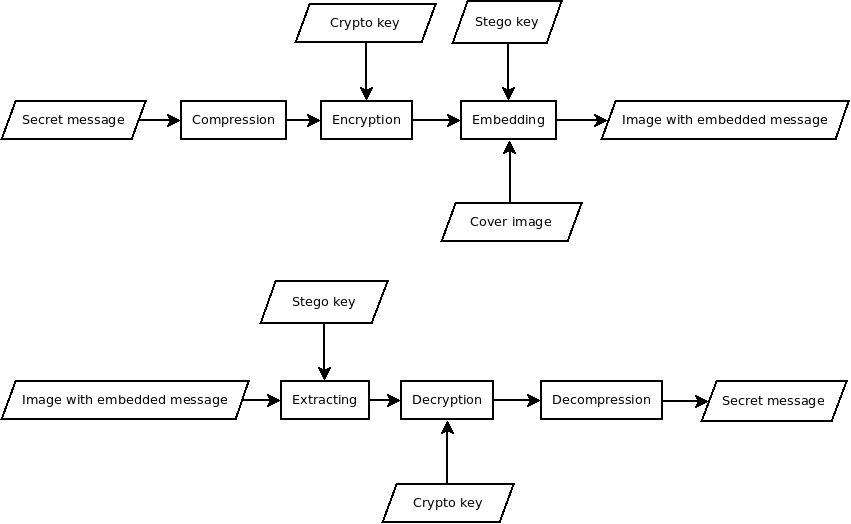
\includegraphics[width=\textwidth]{diagrams/flow.png}}
%popis obrazku
\caption[Main pipelines]{Main pipelines. Upper part: embedding process, lower part: extracting process}
%id obrazku, pomocou ktoreho sa budeme na obrazok odvolavat
\label{img:CSflow}
\end{figure}


\section{Used algorithms}
In this section we will describe algorithms that we used in our application
and discuss their suitness for our purpose. 
We have had to find a balance between potential quality of the algorithms 
and the cost of their implementation and usage.

\textit{We'd like to mention that these algorithms are not the product of our work.}

\subsection{Steganographic algorithm: Complementary embedding (CE)}
\label{ssec:ce}

This algorithm was proposed by Chiang-Lung~Liu and Shiang-Rong~Liao in \cite{liu2008high}.
We've chosen this algorithm as it has better steganographic properties than the ``unofficial
stadnart'' algorithm F5 and is relatively simple to implement and to verify its correctness.

This algorithm was primarily developed to withstand S-attacks (as opposed to F5~algorithm).
It achieves this goal by dividing both message and DCT~coefficients into two parts
(according to steganographic~key and predefined separation~ratio~$\alpha$) and
modifying coefficients in the first part by subtracting and in the second part by addition.

\subsubsection{Embedding process}
\label{sssec:therory-embedding}
Input for the algorithm:

\begin{itemize}
    \item $K$ steganographic key (seed for random generator)
    \item $B$ bytes to be embedded (secret message, encrypted and compressed)
    \item $\alpha$ separation ratio
    \item $\beta$ adjustment parameter
    \item $D$ quantized DCT coefficients sequence
\end{itemize}

Output of the algorithm:

\begin{itemize}
    \item $D'$ changed quantized DCT coefficients
\end{itemize}

\begin{Algo}
\item 
Use a stego-key $K$ to create a permutation of quantized coefficients $D$.
That is, $$Q := P_K(D),$$ where $P(\cdot)$ is a key-dependent
permutation function and $Q$ denotes the permuted coefficient sequence.
\item
Divide $Q$ into two parts, $Q_1$ and $Q_2$, according to separation ratio $\alpha$.
That is, $$Q_1 := Q[0 : \alpha L(Q)],~ Q_2 := Q[\alpha L(Q) : L(Q)],$$
where $L(\cdot)$ denotes the length and $Q[a : b]$ denotes a slice of an array from 
$a$-th to $b$-th element (half-open interval, i.e. $b$-th element does not belong into slice).
\item 
Separate the secret message bytes sequence $B$ into to two parts $B_1$ and $B_2$, 
according to the separation ratio $\alpha$ (similarly to previous step).
\item
Let $L_1$ and $L_2$ denote the byte representations of $L(B_1)$ and $L(B_2)$, respectively.
Let $M_1$ be the concatenation of the $L_1$ and $B_1$ ($M_1 := L_1 || M_1$). Similarly, let
$M_2 := L_2 || B_2$. That would be our two parts we will embed into the cover image.
\item
Convert byte sequences $M_1$ and $M_2$ to bit sequences $M'_1$ and $M'_2$ (by using little endian
encoding).
\item
Embed $M'_1$ into the non-zero coefficients of $Q_1$ using algorithm E1. Note that
the adjustment parameter $\beta$ is used here to make it more resistable against statistical attacks.
\item
Embed $M'_2$ into the non-zero coefficients of $Q_2$ using algorithm E2.
\item
Combine $Q_1$ and $Q_2$ to form a single coefficient sequence $Q'$.
\item 
Using stego-key $K$, depermute the coefficient sequence $Q'$ into $D'$. That is,
$$D' := P^{-1}_K(Q'),$$ where $P^{-1}$ denotes the inverse permutation.
\item 
Return $D'$.
\end{Algo}

Algorithms E1 and E2 are essentially just for-loops through all bits of the secret message
and coefficients with a complex if-statement inside, descibing how to change coefficients
(changes of coefficients depend on oddness of the coefficient and
value of the secret bit). Detailed pseudocode can be found in the original paper \cite{liu2008high}.

Here we show our implementation of these algorithms' if-statements 
in a single function (in Java programming language). 
Variable~$type$ denotes whether we are using E1 or E2 algotithm.

\begin{lstlisting}
public int embedBitUnsafe (final int type, final int c, final int bit) {
    // type: 1 for E1, 2 for E2 algorithm
    // c: (non-zero) coefficient we are changing
    // bit: secret bit to embed
    if (type == 1) {
        if (c > 0 && isOdd(c)) {
            if (bit == 0 && c-1 == 0) return c-2;
            else if (bit == 0 && c-1 != 0) return c-1;
            else if (bit == 1) return c;
        }
        else if (c > 0 && isEven(c)) {
            if (bit == 1) return c-1;
            else if (bit == 0) return c;
        }
        else if (c < 0 && isOdd(c)) {
            if (bit == 1) return c-1;
            else if (bit == 0) return c;
        }
        else if (c < 0 && isEven(c)) {
            if (bit == 0) return c-1;
            // in paper the condition is (c == 1), but it doesn't make much sense
            else if (bit == 1) return c;
        }
    }
    else if (type == 2) {
        if (c > 0 && isOdd(c)) {
            if (bit == 1) return c+1;
            else if (bit == 0) return c;
        }
        else if (c > 0 && isEven(c)) {
            if (bit == 0) return c+1;
            else if (bit == 1) return c;
        }
        else if (c < 0 && isOdd(c)) {
            if (bit == 0 && c + 1 == 0) return c+2;
            else if (bit == 0 && c + 1 != 0) return c+1;
            else if (bit == 1) return c;
        }
        else if (c < 0 && isEven(c)) {
            if (bit == 1) return c+1;
            else if (bit == 0) return c;
        }
    }
}
\end{lstlisting}

Algorithm E1 additionally change a part of used coefficients using the adjustment
parameter $\beta$. The adjustment is simple: we need to look at first $\beta L(M)$ coefficients and
change values $-2$ to value $1$.

\subsubsection{Extraction process}
Input for the algorithm:

\begin{itemize}
    \item $K$ steganographic key (seed for random generator)
    \item $\alpha$ separation ratio
    \item $D$ quantized DCT coefficients sequence with embedded message
\end{itemize}

Output of the algorithm:

\begin{itemize}
    \item $B$ extracted bytes of the secret message
\end{itemize}

\begin{Algo}
\item 
Use a stego-key $K$ to create a permutation of quantized coefficients $D$.
That is, $$Q := P_K(D),$$ where $P(\cdot)$ is a key-dependent
permutation function and $Q$ denotes the permuted coefficient sequence.
\item
Divide $Q$ into two parts, $Q_1$ and $Q_2$, according to separation ratio $\alpha$.
That is, $$Q_1 := Q[0 : \alpha L(Q)],~ Q_2 := Q[\alpha L(Q) : L(Q)],$$
where $L(\cdot)$ denotes the length and $Q[a : b]$ denotes a slice of an array from 
$a$-th to $b$-th element (half-open interval, i.e. $b$-th element does not belong into slice).
\item
Extract the length $L_1$ of the embedded message from the $Q_1$, then extract $8 L_1$ bits of
the embedded message $B'_1$ from $Q_1$ by using the following algorithm:
\begin{lstlisting}
if (c > 0 && isEven(c)) return 0;
if (c < 0 && isOdd(c))  return 0;
if (c > 0 && isOdd(c))  return 1;
if (c < 0 && isEven(c)) return 1;
\end{lstlisting}
\item
Similarly, extract the length $L_2$ of the embedded message from $Q_2$ and $8 L_2$ bits of the 
embedded message $B'_2$ by using the following algorithm:
\begin{lstlisting}
if (c > 0 && isOdd(c))  return 0;
if (c < 0 && isEven(c)) return 0;
if (c > 0 && isEven(c)) return 1;
if (c < 0 && isOdd(c))  return 1;
\end{lstlisting}
\item
Convert bit sequences of the secret messages $B'_1$ and $B'_2$ to byte sequences $B_1$ and $B_2$.
\item
Combine $B_1$ and $B_2$ into single secret message $B$.
\item 
Return $B$.

\end{Algo}

\subsubsection{Tuning the parameters $\alpha$ and $\beta$}
The original paper suggests that the separation ratio $\alpha$
should be chosen from a~segment~$\left[ \frac{3}{4}, \frac{5}{6} \right]$
and the adjustment parameter $\beta$ should be chosen from a~segment~$\left[\frac{1}{8}, \frac{1}{3}\right]$ 
(bigger $\beta$ positively correlates with
better undetectability of the message). 
In tests the authors have chosen
values $\frac{4}{5}$ and $\frac{1}{3}$, respectively.

\subsubsection{Limit for a message length}
The authors of the algorithm implies that for chosen values of the parameters
it is safe enough to use even $50\%$ of nonzero coefficients, i.e. the algorithm
is still resistable to chi-square and S families of attacks. As for general measures
of changing of the cover image, authors tell us that it is safe enough to use all
nonzero coefficients available.

\subsection{Cryptographic algorithm: AES}

We are using AES-256-CBC algorithm for encryption. It is a current standart
solution for symmetric encryption. The algorithm is described here \cite{standard2001announcing}.

One of the main problems of cryptography is a big chance to use it incorrectly.
Therefore, we've decided to use an open implementation of it, provided by the package
\texttt{com.scottyab.aescrypt.AESCrypt}. 


\subsection{Compression algorithm: GZIP}
We are using GZIP algorithm mainly because it has been implemented in standard
Java library as \texttt{java.util.zip.GZIPInputStream} and 
\texttt{java.util.zip.GZIPOutputStream} classes. This compression
is based on widely used algorithm DEFLATE, which is based on Huffman encoding and LZ77 algorithm.
You can read more about this in \cite{deutsch1996deflate} and \cite{deutsch1996gzip}.

\section{Resistance against additional compression}
\label{sec:addcomp}

In this section we will shortly decribe the possibilities of compression-resistant
steganography.

Recompression of a JPEG image has a lot of parameters. Main are the size of an image
and the quality ratio (described in section \ref{sec:jpeg}), but there is a plenty of
secondary ones, like encoding the pixels in RGB or in YCrCb, rounding of Cb and Cr channels
(8 bytes or 4 bytes), and so on.

Good news are that the most of these factors can be dealt with by simply choosing a cover
image with the same parameters as the result of the additional comprimation (assuming 
these parameters aren't going to change).   

The are two problematic ones: the size and the quality ratio, as they could be change
from device to device (e.g. Facebook Messenger generally shows images in better 
quality for Apple smartphones that Android ones). 

We can deal with the size of an image by choosing the one the communication channel 
would use for the given ends of a channel (i.e. the two given mobile phones). Otherwise,
this issue is quite hard to reliably solve, as changing of the size would result in
merging the adjacent blocks of an image, erasing the values of last bits of the DCT coefficients,
ruining any DCT-based steganography.

We can, in theory, deal with the change of quality ratio by using error-correction codes.
The main issue is that lowering of the quality would result in nullifying the coefficients,
thus shifitng the space the algorithm would search for a hidden message. It can be seen
as the erasing of message symbols in general coding theory. It could be dealt with
by permuting the whole blocks, not the individual coefficients.

Another issue is that the error-correction would result in longer message and, therefore,
higher change of detection.

In our application, we decided not to implement the compression-resistant algorithm.

\section{How to use the application correctly}
In this section we will describe common mistakes and give some advices on
how to achieve maximum inconspicuousness.

\subsubsection{Never use the same image twice}

Imagine a situation: the censor sees two visually identical message with little 
differencies in thier digital representation. He may make only one conclusion: 
the sender tries to manipulate the images to send some information. Therefore
it is highly unrecommended to use similar images to steganography.

\subsubsection{Never send the same message twice}

Imagine another situation: the censor sees two images, compare their DCT coefficients
and sees the the pattern in their last bits (remember, the secret bits are embedded into
the same positions). There is only one natural conclusion: the sender uses the steganography.

\subsubsection{Use images with high number of colours}
Also avoid computer art, images with semantic context (like texts).

\subsubsection{Change your keys frequently}
Firstly, the keys have tendency to be leaked. Secondly, with enough tapped communication,
keys can be deduced with prior knowledge. Thirdly, modern stochastic statistical approaches 
(neural networks, nonlinear programming, etc.) could theoretically distinguish images with
embedded messages from ``clean'' even without any knowledge of the algorithm, not mentioning
the keys. Fixing the key (i.e. fixing the positions of the cofficients to be changed)
would only help the attackers.


\subsubsection{Generate your secret keys by app's utilities, not by hand}
Another general advice: small human-generated passwords are easier to break (dictionary attack,
bruteforce, etc.). All basic advices for choosing a password are applicable here: long passwords
with nonstandard symbols (numbers, special symbols, uppercase, etc.) are generally better.

We recommend to use standard in-app utility to generate the keys.

If you decide to generate the password by yourself, 
we recommend to stay in a set of ASCII characters for simplier key distribution (although keys are
stored as UTF-8 strings, so you can potentially use even non-latin symbols 
(Japan hieroglyphs, Arabic symbols, cyrillic, etc.)).

\subsubsection{Use only secure channels to distribute your keys}
The best option is to physically meet with your correspondent.


\subsubsection{Try to write your messages as short as possible}
This rule has a simple explanation: shorter message means less changed coefficients, thus
lesser distortion in statistical properties of an image, therefore better undetectability.
We recommend to send messages with length less than 1kB (based on claimed effectiveness
of steganalytic methods).

\subsubsection{Use only lossless communication channels}
As described in the section \ref{sec:addcomp}, additional compression could and probably
would destroy the hidden message. There are many lossless channels: e-mail, Dropbox, Google Drive,
Google Photos, Telegram messenger, Skype, etc.
